\section{Results}

% \begin{itemize}
%     \item Methods on how we're doing simulations and results (with simulations and experimental data)
%     \begin{itemize}
%         \item Different SNRs and maybe even use CAPs
%         \item Selection of HRF explained if both use the same but it's different from what's used for simulating.
%         \begin{itemize}
%             \item What happens? For example with gamma for simulating.
%         \end{itemize}
%         \item Selection of regularization parameter
%         \begin{itemize}
%             \item Present with real data on a voxel
%         \end{itemize}
%     \end{itemize}
% \end{itemize}

A critical decision with deconvolution methods is the selection of the regularization parameter \(\lambda\), for which many techniques have been proposed in the literature but an optimal is yet to be discovered. In fact, Paradigm Free Mapping and Total Activation base their selection of the regularization parameter on different criteria: the Bayesian Information Criterion (BIC) (\citealt{schwarz1978EstimatingDimensionModel}), and a selection based on the convergence of the residuals to a pre-estimated level of the noise, respectively. Hence, we compare the performance of the two algorithms with both selection criteria. Furthermore, we explore the differences between the techniques in terms of the estimation of the activity-inducing signal \(\mathbf{s}\) using the \textit{spike model} in~\eqref{eq:pfm_spike} and the innovation signal \(\mathbf{u}\) using the \textit{block model} in~\eqref{eq:pfm_block}.

\subsection{Selection of the hemodynamic response function}

With the aim of making a fair comparison of the two methods, we first compared their hemodynamic response functions. Figure~\ref{fig:hrf_diff}A shows the difference in the hemodynamic response function that PFM and TA use by default for TR = 0.1 s and TR = 1 s adjusted to peak amplitude of one; i.e., the canonical HRF and the HRF resulting from the linear differential operator. The most observable difference between the two HRFs is the time to peak: the HRF used by Total Activation does not begin at zero while the one used by PFM does.

\begin{figure}[h]
    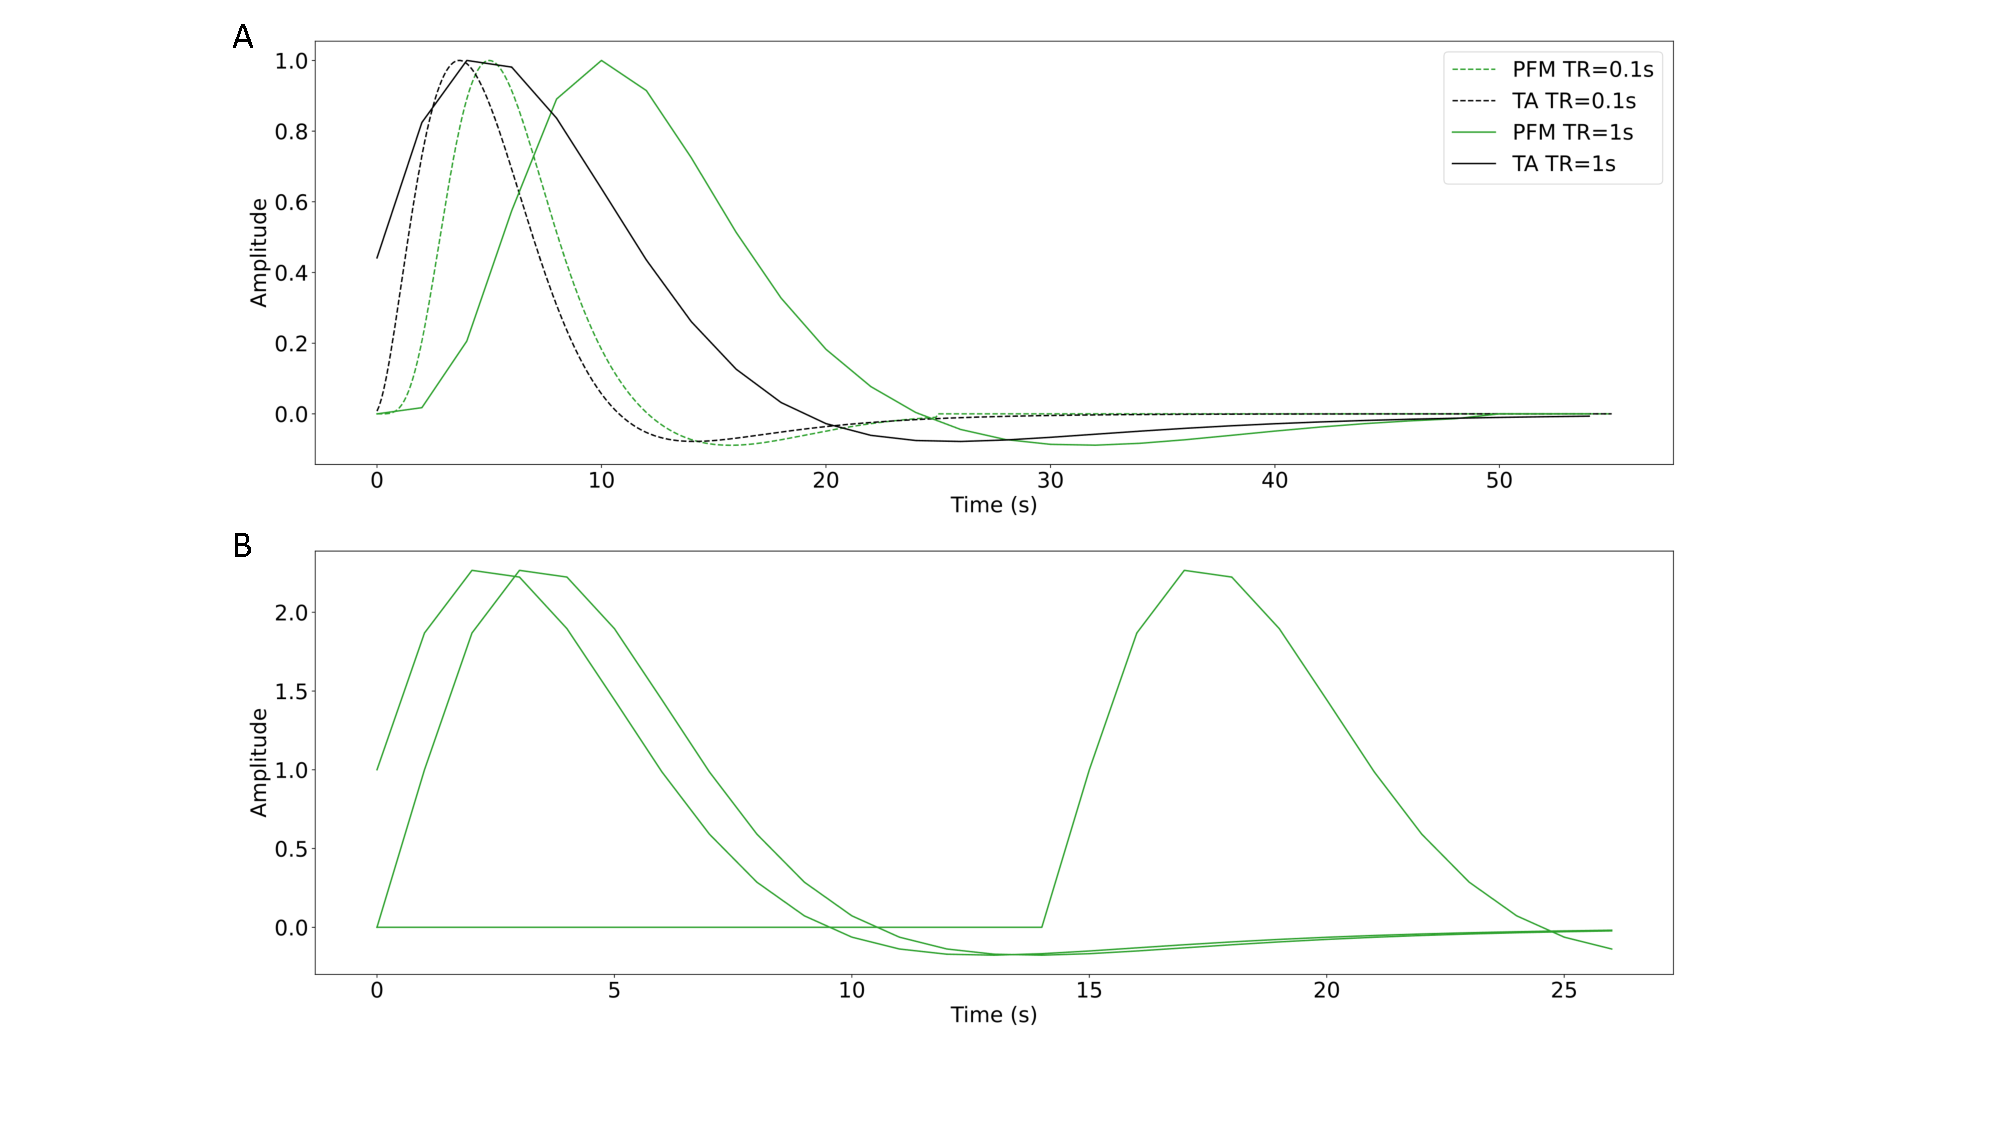
\includegraphics[width=\columnwidth]{figures/pfm_ta_hrf.pdf}
    \caption{A) Canonical HRF models typically used by PFM (green) and TA (black) at TR = 0.1 s (dashed lines) and TR = 1 s (solid lines). Without loss of generality, the waveforms are scaled to unit amplitude for visualization. B) Representation of three shifted HRFs at TR=1 s (onsets=0, 1, and 15 s) that build the design matrix for PFM when the HRF model has been matched to that in TA.}
\label{fig:hrf_diff}
\end{figure}

While Paradigm Free Mapping allows for the use of any hemodynamic response function --- the columns of the design matrix \(\mathbf{H}\) are composed by shifted versions of the HRF--- the linear differential operator in TA is tailored for a fixed HRF. Hence, for practical reasons, we reproduced the HRF in the Total Activation filter and incorporated it into the PFM formulation (Figure~\ref{fig:hrf_diff}B).

\subsection{Selection of the regularization parameter based on the estimation of the noise}

\begin{figure*}[t!]
    \begin{center}
        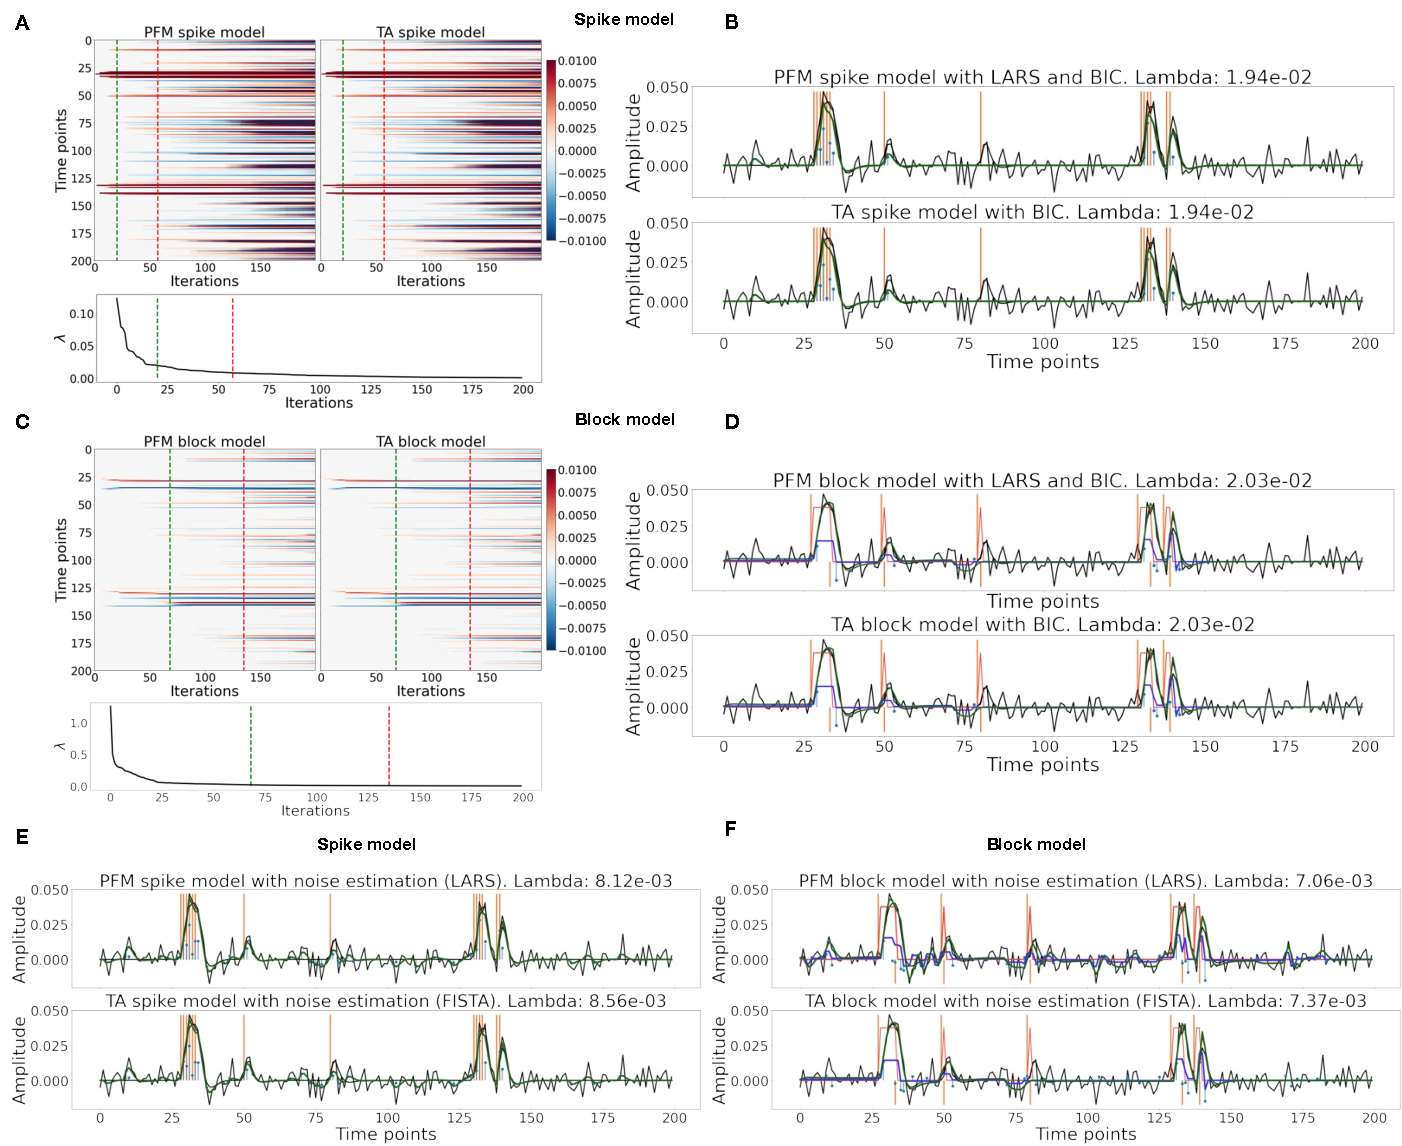
\includegraphics[width=\textwidth]{figures/figure_sim.pdf}
    \end{center}
    \caption{A) (Left) Heatmap of the regularization paths of the activity-inducing (top) and innovation (bottom) signals estimated with PFM and TA as a function of \(\lambda\) for the simulated data with SNR = 3 dB (x-axis: increasing number of iterations or \(\lambda\) as given by LARS; y-axis: time; color: amplitude). Vertical lines denote iterations corresponding to the Akaike and Bayesian Information Criteria (AIC and BIC) optima. (Right) Estimated activity-inducing (blue) and activity-related (green) signals \(\lambda\) is selected based on BIC. B) Estimated activity-inducing, innovation and activity-related (fit, \(\mathbf{x}\)) signals when \(\lambda\) is selected based on the MAD method with the spike model (left, with PFM on the left and TA on the right) and block model (right, with PFM on the left and TA on the right) for the simulated data with SNR = 3 dB.}
\label{fig:sim}
\end{figure*}

% \begin{figure*}[t!]
%     \begin{center}
%         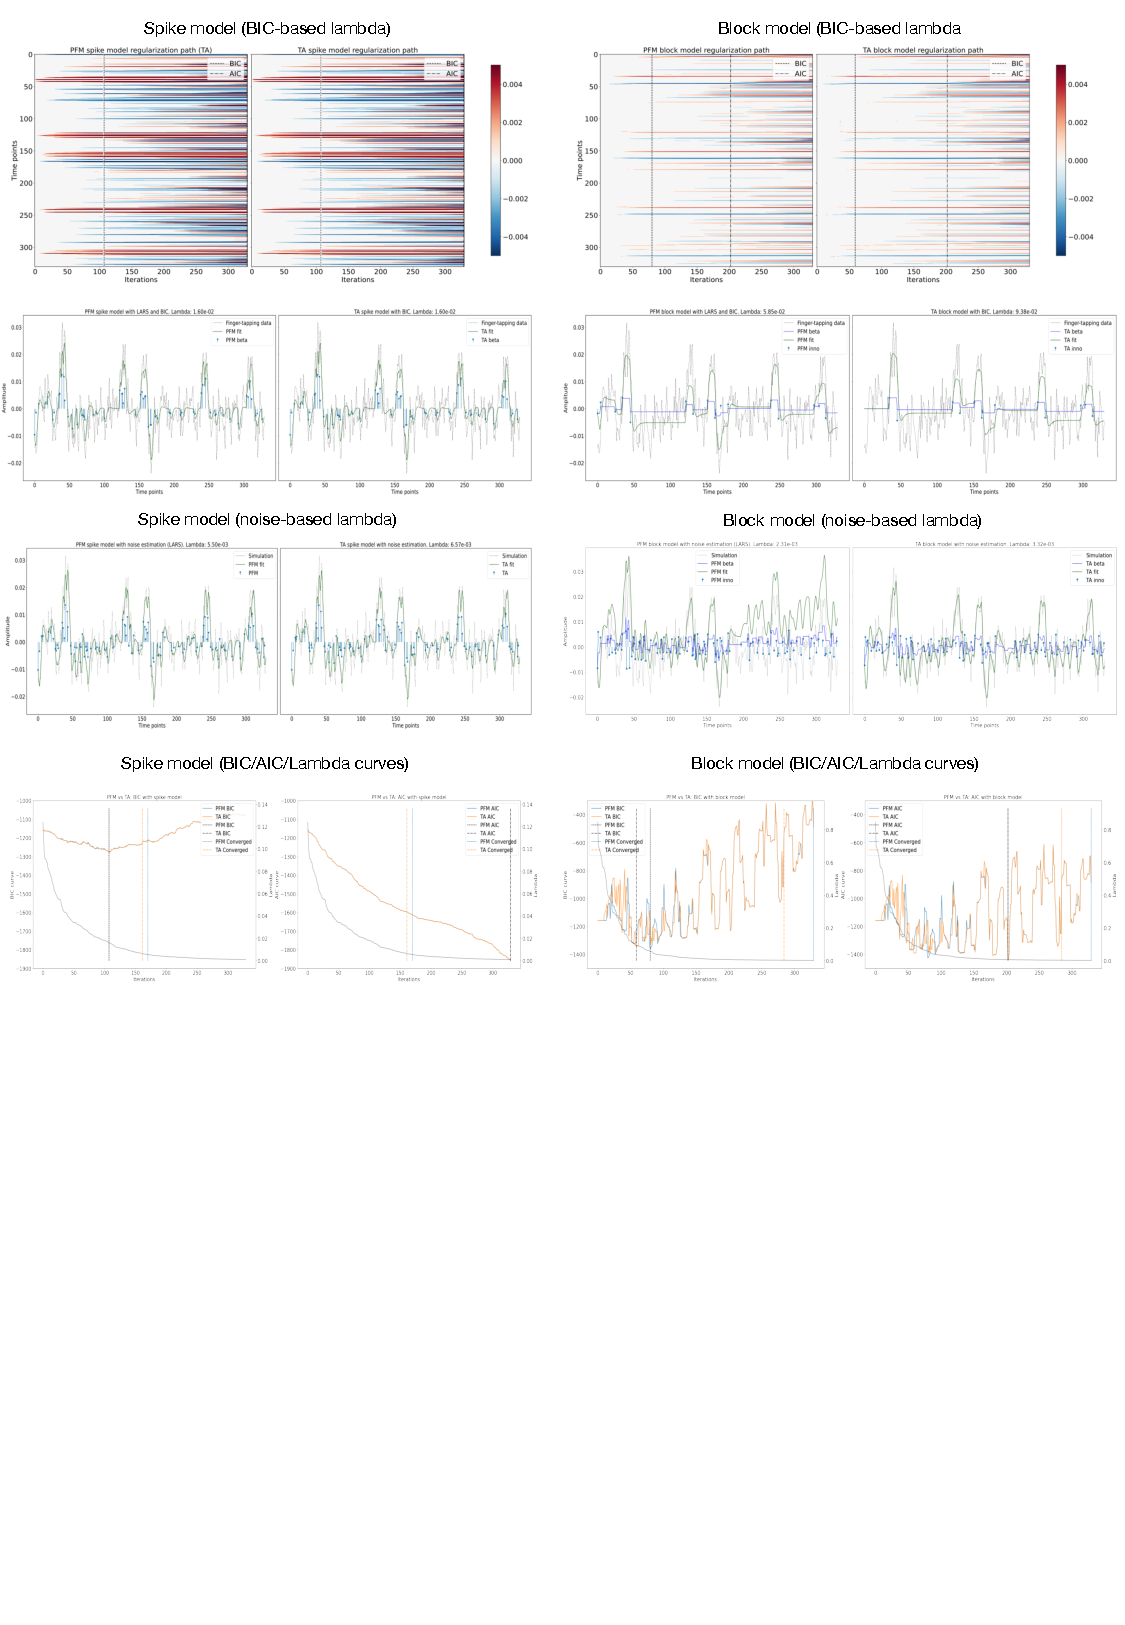
\includegraphics[width=\textwidth]{figures/exp.pdf}
%     \end{center}
%     \caption{(Row 1) Regularization paths of the estimated activity-inducing signal (spike model --- left) and innovation signal (block model --- right); (Row 2) activity-inducing, innovation and activity-related (fit, \(\mathbf{x}\)) signals when \(\lambda\) is selected based on BIC, or (Row 3) based on convergence of residuals to have same variance as MAD estimate of noise; (Row 4) Corresponding cost curves of BIC and AIC. The vertical lines indicate the three options to select \(\lambda\) (BIC, AIC and Converged/MAD).}
% \label{fig:exp}
% \end{figure*}

Total Activation proposes to solve the inverse problem by updating the regularization parameter \(\lambda\) on every iteration \(n\) so that the residuals converge to a previously estimated noise level of the data fit \(\tilde{\sigma}\), where this pre-estimated noise is calculated from the median absolute deviation of fine-scale wavelet coefficients (Daubechies, order 3) (\citealt{karahanoglu2013TotalActivationFMRI}):

\begin{equation}
    \lambda^{n+1} = \frac{N \tilde{\sigma}}{\frac{1}{2} \| \mathbf{y} - \mathbf{x}^n \|_F^2} \lambda^n.
\label{eq:std}
\end{equation}

Thus, we calculated the regularization path with PFM (as described in \ref{sec:regpath}) and selected the \(\lambda\) corresponding to the residuals that were closest to the estimated noise level of the data. We applied Total Activation with temporal regularization in its original form. Figure~\ref{fig:sim}B depicts the estimated activity-inducing, innovation, and activity-related signals when updating \(\lambda\) following~\eqref{eq:std} in the three simulated SNR settings using the spike model (left) and the block model (right). Figure~\ref{fig:sim}B (left) shows nearly identical results between PFM (left) and TA (right) with the use of the spike model. The minimal differences are the result of slight dissimilarities in the convergence of the residuals to the estimated noise level of the data. Likewise, the use of the block model with a selection of \(\lambda\) based on the MAD estimate of the noise yields results that are identical in practice as shown in Figure~\ref{fig:sim}B (right).

\subsection{Selection of the regularization parameter by solving the regularization path}
\label{sec:regpath}

\begin{figure*}[t!]
    \begin{center}
        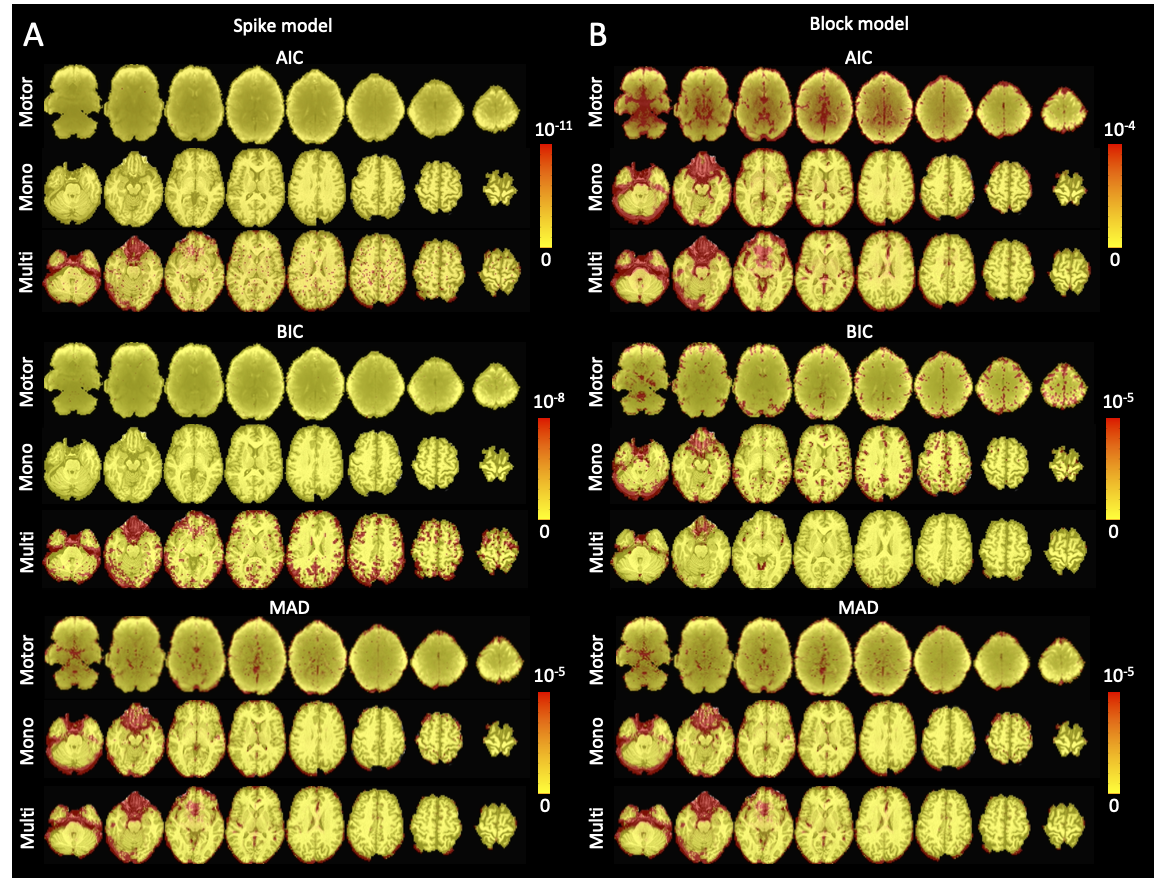
\includegraphics[width=\textwidth]{figures/maps.pdf}
    \end{center}
    \caption{Sum of squares of the differences of the activity-inducing signals estimated with Paradigm Free Mapping and Total activation for the different selections of the regularization parameter: BIC (top), and MAD (bottom). The sum of square difference maps are shown for the three experimental datasets introduced in Section~\ref{sec:data}: the motor task (Motor), the monoband resting-state (Mono), and the multiband resting-state (Multi) datasets. A) Sum of squares of the differences when using the spike model. B) Sum of squares of the differences when using the block model.}
\label{fig:rss}
\end{figure*}

Paradigm Free Mapping bases its selection of the regularization parameter on the BIC. Hence, we calculated the regularization path with PFM by means of the least angle regression (LARS) algorithm (\citealt{efron2004LeastAngleRegression}) and used the \(\lambda\)s from the regularization path to solve the deconvolution problem with Total Activation.

Figure~\ref{fig:sim}A (left) shows the regularization paths of PFM and TA side by side for the three SNR conditions for the spike model; i.e., the inverse problem described in~\eqref{eq:pfm_spike}. Each iteration of LARS reduces the value of \(\lambda\); i.e., reduces the sparsity promoted by the \(l_1\)-norm, and reveals new non-zero coefficients as shown in the x-axis of the heatmaps. Vertical black lines depict the selection of the regularization parameter based on BIC, and thus, the colored coefficients indicated by the vertical lines depict the estimated activity-inducing signal \(s(t)\). Figure~\ref{fig:sim}A (right) illustrates the resulting estimation of the activity-inducing and neuronal-related signals when basing the selection of \(\lambda\) on BIC for the three simulated SNR conditions. Given that the regularization paths of both techniques are identical, the BIC-based selection of the regularization parameter and the results of deconvolving with said \(\lambda\) are identical too (see Figure~\ref{fig:lambdas}). Thus, Figure~\ref{fig:sim}A demonstrates that, regardless of the simulated SNR condition, both deconvolution algorithms produce identical regularization paths when the same HRF and regularization parameters are applied, and hence, identical estimates of the activity-inducing signal \(\mathbf{s}\) and neuronal-related signal \(\mathbf{x}\).

The regularization path to estimate innovation signals yields mainly undistinguishable results for both PFM and TA methods as shown in Figure~\ref{fig:sim}A (left). Again, the BIC-based selection of \(\lambda\) is identical for both PFM and TA, and the estimation of the innovation signal \(\mathbf{u}\) shows no distinguishable differences between the algorithms (see Figure~\ref{fig:sim}A right). Therefore, both Paradigm Free Mapping and Total Activation yield nearly identical regularization paths and estimates of the innovation signal regardless of the simulated SNR condition when applying the same HRF and regularization parameters with the block model.

% Furthermore, we performed the same analysis on experimental data as shown in Figure~\ref{fig:exp} (rows 1-2, 4). Row 1 demonstrates that the PFM and TA regularization paths are identical when deconvolving experimental data, regardless of the deconvolution model (spike or block). Even though tiny differences can be seen between the two methods in the BIC selection of \(\lambda\) in row 4, row 2 proves that the results are practically identical, and differences can be disregarded.

\subsection{Performance on experimental data}

Additionally, in order to describe the extent of the discrepancies between the techniques, we calculated the residual sum of squares (RSS); i.e., the sum of squares of the differences between the estimated activity-inducing or innovation signals of PFM and TA as:
\begin{equation}
    RSS = \frac{\sum{(\hat{s}_{PFM} - \hat{s}_{TA})^2}}{N}.
\end{equation}

Figure~\ref{fig:rss} depicts the RSS of the spike (Figure~\ref{fig:rss}A) and block (Figure~\ref{fig:rss}B) models for the three experimental datasets introduced: i.e., motor, monoband and multiband. It is clear that RSS values are lower than those of the activity-inducing and innovation signals, suggesting that the differences between Paradigm Free Mapping and Total Activation are negligible. Furthermore, the largest differences can be seen in regions with high vasculature and are probably a result of differences in the amplitude of the estimated activity-inducing and innovation signals.
